\subsection{Probabilistic Payment Channels}
\label{sec:incentives:probabilistic}

TODO: add polish paper

\begin{figure}[H]
    \centering
    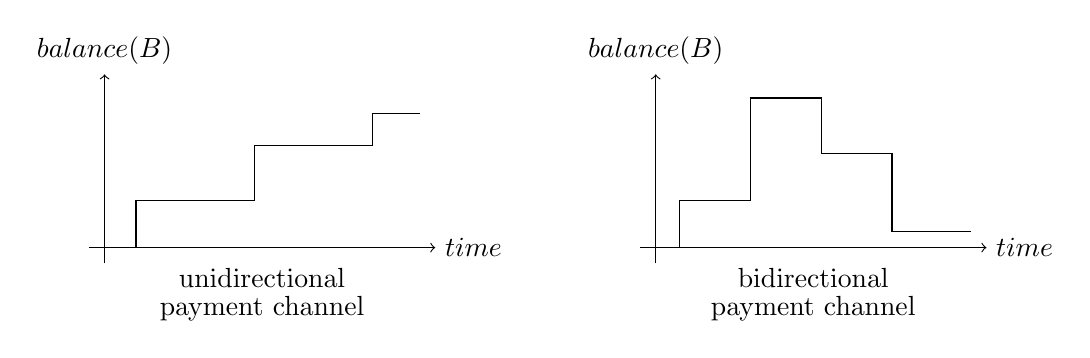
\begin{tikzpicture}[domain=0:2]
        \def\padding{0.1}
        \def\plotHeight{2}
        \def\plotWidth{4}
        \def\plotOffset{7}
        \def\textOffset{0.6}
        \foreach \i in {0,1} {
                \begin{scope}[shift={(\i*\plotOffset,0)}]
                    \draw[->] (-2*\padding,0) -- (\plotWidth+2*\padding,0) node[right] {$time$};
                    \draw[->] (0,-2*\padding) -- (0,\plotHeight+2*\padding) node[above] {$balance(B)$};

                    \ifnum\i=0
                        \path (0,-\textOffset) -- (\plotWidth,-\textOffset) node[midway] {\shortstack{unidirectional\\payment channel}};
                        \draw (0.4,0) -- (0.4,0.6) -- (1.4,0.6) -- (1.9,0.6) -- (1.9,1.3) -- (2.6,1.3) -- (3.4,1.3) -- (3.4,1.7) -- (4.0,1.7);
                    \else
                        \path (0,-\textOffset) -- (\plotWidth,-\textOffset) node[midway] {\shortstack{bidirectional\\payment channel}};

                        \draw (0.3,0) -- (0.3,0.6) -- (1.2,0.6) -- (1.2,1.9) -- (2.1,1.9) -- (2.1,1.2) -- (3.0,1.2) -- (3.0,0.2) -- (4.0,0.2);
                    \fi
                \end{scope}
            }
    \end{tikzpicture}
    \label{fig:channels}
    \caption{Node $A$ and $B$ have a payment channel. Whilst in case of unidirectional payment channels, $balance(B)$ is strictly increasing, the derivative of $balance(B)$ \textit{can} change sign if the channel is bidirectional.}
\end{figure}

\begin{figure}[H]
    \centering
    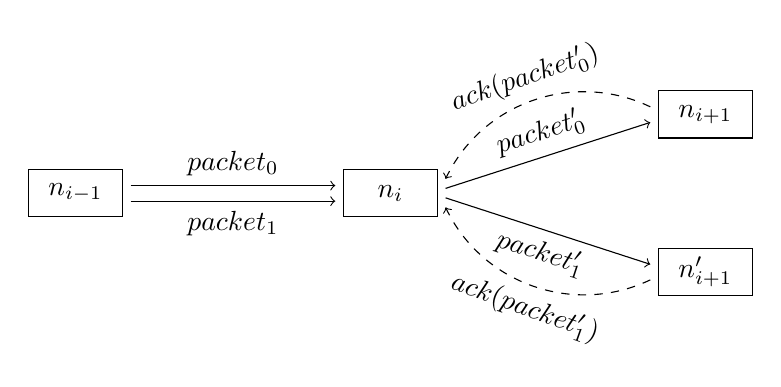
\begin{tikzpicture}
        \def\nodeOffset{4}
        \def\nodeYOffset{1}
        \def\nodeWidth{1.2}
        \def\nodeHeight{0.6}
        \def\padding{0.1}

        \foreach \xOffset\yOffset\name in{-\nodeOffset/0/$n_{i-1}$,0/0/$n_i$,\nodeOffset/\nodeYOffset/$n_{i+1}$,\nodeOffset/-\nodeYOffset/$n_{i+1}'$} {
                \draw[shift={(\xOffset,\yOffset)}] (0,0) rectangle (\nodeWidth,\nodeHeight) node[midway] {\name};
            }

        % Packets
        \draw[->,shift={(0,0.66*\nodeHeight)}] (-\nodeOffset+\nodeWidth+\padding,0) -- (-\padding,0) node[midway,above] {$packet_0$};
        \draw[->,shift={(0,0.33*\nodeHeight)}] (-\nodeOffset+\nodeWidth+\padding,0) -- (-\padding,0) node[midway,below] {$packet_1$};

        % Forwarded packets
        \draw[->] (\nodeWidth+\padding,0.6*\nodeHeight) -- (\nodeOffset-\padding,\nodeYOffset+0.33*\nodeHeight) node[midway,sloped,above] {$packet_0'$};
        \draw[->] (\nodeWidth+\padding,0.4*\nodeHeight) -- (\nodeOffset-\padding,-\nodeYOffset+0.66*\nodeHeight) node[midway,sloped,below] {$packet_1'$};

        % Acknowledgements
        \draw[->,dashed] (\nodeOffset-\padding,\nodeYOffset+0.66*\nodeHeight) to [bend right=45] node[above,sloped] {$ack(packet_0')$} (\nodeWidth+\padding,0.8*\nodeHeight);
        \draw[->,dashed] (\nodeOffset-\padding,-\nodeYOffset+0.33*\nodeHeight) to [bend left=45] node[below,sloped] {$ack(packet_1')$} (\nodeWidth+\padding,0.2*\nodeHeight);
    \end{tikzpicture}
    \caption{Node $n_{i-1}$ send packet $packet_0$, $packet_1$ to node $n_i$ which forwards them to node $n_{i+1}$ and node $n_{i+1}'$. Both nodes acknowledge the validity of $packet_0'$ and $packet_1'$ to node $n_i$.}
    \label{fig:sharedpaymentchannel}
\end{figure}

% Use data structure tickets

% Steady payments, expect continuous payments

% Entropy

% Continuous payments

\paragraph{Payment channels}

In traditional payment channels, two parties $A$ and $B$ lock some funds within a smart contract, make transactions off-chain and only commit the aggregation on-chain.



Thus, a payment channel is bidirectional, which means both $A$ and $B$ can send and receive transactions within the same payment channel. The HOPR protocol uses unidirectional payment channels to implement bidirectional payment channel behaviour, where one payment channel is created from $A$ to $B$ and another from $B$ to $A$. The payment channel creator is the sole owner of funds in the payment channel and the only one able to create \textbf{tickets}, encapsulated funds which are described in detail in Section \ref{sec:tickets}. A payment channel created from party $A$ to party $B$ is different from a payment channel created from party $B$ to party $A$.

$$A\rightarrow B \neq B\rightarrow A$$

\paragraph{Probabilistic payments}

This separation reflects the directional nature of packets flowing through the network. It also brings the advantage that each payment channel's logic is easier to verify.

\paragraph{Wrap Up}

\paragraph{Acknowledgements} are messages which allow every node to acknowledge the processing of a packet to the previous node. This acknowledgement ($ACK$) contains the cryptographic material needed to unlock the possible payout for the previous node. Note that an acknowledgement is always sent to the previous node, and using acknowledgments with vanilla payment channels results in accumulated incentives, where the latest acknowledgement contains all previous incentives plus the incentive for the most recent interaction, as explained below:

\begin{align}
    value (ACK_n) & =\sum_{i=1}^nfee_{packet_i},
\end{align}
where $n$ is the total number of mixnet packets transformed.

An issue arises when $B$ receives $ACK_n$ for $packet_n$ before sending $packet_{n-1}$. At this point $B$ would have no incentive to process $packet_{n-1}$ rather than $packet_{n}$. To avoid such false incentives, the HOPR protocol utilizes probabilistic payments. A \textit{ticket} can be either a win or a loss, determined based on some winning probability lower than 1. This means nodes are incentivized to continue relaying packets, as they do not know which tickets will result in a payout. From a node's perspective, each ticket has the same value until it is claimed; therefore, the HOPR protocol encourages nodes to claim tickets independently from each other.

\begin{align}
    value ( ACK_i ) & =value ( ACK_j ) \quad for \quad i,j\in \{1,\dots,n\}
\end{align}

If we assume constant costs, there is no added value in pretending packet loss or intentionally changing the order in which packets are processed. On the contrary, a node would reduce its potential payouts if it were to forward packets slowly or not at all.